% ══════════════════════════════════════════════════════════════════════
% BENCHMARK DATASET STATISTICS
% Input this file after \section{Benchmark Scenarios and Instantiations}
% ══════════════════════════════════════════════════════════════════════

\subsection{Dataset Statistics}
\label{sec:dataset-stats}

We instantiated EABench across three concrete tenant organizations spanning distinct enterprise domains: a boutique law firm (\emph{Bertrand \& Co.}, 41 users), a mid-size research university (\emph{University of Cambford}, 62 users), and a fast-growing AI startup (\emph{ZAI Intelligence}, 165 users). Each tenant was generated independently by the same GPT-4o-based pipeline described in Section~\ref{sec:method_generation}, parameterized with a domain-specific company description, a set of key narrative events, and an organizational size. The staged generator ensures that artifacts within a single simulated day are mutually coherent---an email thread's content is consistent with the meeting that prompted it---while still allowing realistic variation across days.

Table~\ref{tab:dataset_summary} summarizes the resulting artifact counts and evaluation-case distribution. For each tenant, three evaluation query generators---targeted artifact search, multi-hop reasoning, and comprehensive report---produce structured test cases in a separate pass that examines the completed corpus and constructs questions, gold assertions, and entity lists against it.

\begin{table*}[t]
\centering
\caption{Artifact composition and evaluation case counts for the three EABench tenants.
For chats and group chats, the count reflects distinct conversation threads rather than individual messages.
Evaluation cases span targeted artifact search, multi-hop reasoning, and comprehensive report query types (see Section~\ref{sec:eval-metrics}).}
\label{tab:dataset_summary}
\small
\resizebox{\textwidth}{!}{%
\begin{tabular}{lcccccccccc}
\toprule
\textbf{Tenant} & \textbf{Domain} & \textbf{Users} & \textbf{Emails} & \textbf{DMs} & \textbf{Group} & \textbf{Meetings} & \textbf{Files} & \multicolumn{3}{c}{\textbf{Eval Cases}} \\
\cmidrule(lr){9-11}
 & & & & & \textbf{Chats} & & & \textbf{Tgt.\ Search} & \textbf{Multi-Hop} & \textbf{Compreh.} \\
\midrule
Bertrand \& Co.     & Legal       & 41  & 132 & 56  & 118 & 69  & 70  & 80 & 43 & 39 \\
Univ.\ of Cambford  & Education   & 62  & 120 & 41  & 118 & 70  & 70  & 80 & 44 & 38 \\
ZAI Intelligence    & AI / SW     & 165 & 298 & 140 & 301 & 164 & 164 & 79 & 82 & 40 \\
\midrule
\textbf{Total}      &             & 268 & 550 & 237 & 537 & 303 & 304 & 239 & 169 & 117 \\
\bottomrule
\end{tabular}}
\end{table*}

\noindent The three tenants vary substantially in scale: ZAI Intelligence is roughly four times larger than Bertrand \& Co.\ across every artifact category, and its eval-case count (201) is proportionally expanded to maintain per-tenant statistical power. This heterogeneity is intentional---EABench is designed to stress-test agents under differing information densities rather than to standardize them away.

The query-type distribution follows the pipeline's target split of approximately 40/40/20 (targeted artifact search / multi-hop reasoning / comprehensive report). The actual ratios deviate slightly because each generator produces variable-sized batches. Targeted artifact search queries each reference exactly one gold entity, multi-hop reasoning queries reference 2--5 entities from different modalities, and comprehensive report queries reference 3--15 entities spanning multiple artifact types and dates.

\begin{table}[h]
\centering
\caption{Ground-truth evaluation complexity by query type and tenant.
``Assertions'' are gold-standard factual statements the agent's response must satisfy;
``Entities'' are the ground-truth artifacts (emails, chats, meetings, files) required to answer the query.}
\label{tab:ground_truth}
\small
\begin{tabular}{llcccccc}
\toprule
& & \multicolumn{3}{c}{\textbf{Assertions per Case}} & \multicolumn{3}{c}{\textbf{Entities per Case}} \\
\cmidrule(lr){3-5} \cmidrule(lr){6-8}
\textbf{Tenant} & \textbf{Query Type} & \textbf{Mean} & \textbf{Med.} & \textbf{Range} & \textbf{Mean} & \textbf{Med.} & \textbf{Range} \\
\midrule
\multirow{3}{*}{Bertrand}
  & Targeted Artifact Search  & 2.4 & 2 & 2--4  & 1.0 & 1 & 1--1  \\
  & Multi-Hop Reasoning        & 2.3 & 2 & 2--3  & 2.7 & 2 & 2--5  \\
  & Comprehensive Report       & 3.2 & 3 & 3--4  & 5.3 & 5 & 4--10 \\
\midrule
\multirow{3}{*}{Cambford}
  & Targeted Artifact Search  & 2.6 & 3 & 2--3  & 1.0 & 1 & 0--1  \\
  & Multi-Hop Reasoning        & 2.8 & 3 & 2--4  & 3.1 & 3 & 2--4  \\
  & Comprehensive Report       & 3.2 & 3 & 3--4  & 5.9 & 5 & 3--15 \\
\midrule
\multirow{3}{*}{ZAI}
  & Targeted Artifact Search  & 2.2 & 2 & 2--3  & 1.0 & 1 & 1--1  \\
  & Multi-Hop Reasoning        & 2.3 & 2 & 2--5  & 2.4 & 2 & 2--5  \\
  & Comprehensive Report       & 3.2 & 3 & 3--4  & 6.0 & 5 & 3--11 \\
\bottomrule
\end{tabular}
\end{table}

\noindent Table~\ref{tab:ground_truth} reveals a clear complexity gradient across query types. Targeted artifact search queries average 2.2--2.6 assertions grounded in a single entity, making them the simplest evaluation targets. Multi-hop reasoning queries maintain a similar assertion count but require cross-referencing 2--5 entities from different communication modalities. Comprehensive report queries demand the most complex synthesis: 3--4 assertions each backed by 3--15 source entities spanning emails, chats, meetings, and files. This structured complexity scaling ensures that the evaluation set probes agent capabilities at multiple difficulty levels.

\subsection{Communication Network Properties}
\label{sec:network-stats}

To characterize inter-personal communication structure, we extract a directed multigraph for each tenant in which nodes are users and edges represent recorded communicative acts across five channel types: email (\emph{from}$\to$\emph{to}), email CC (\emph{from}$\to$\emph{cc}), direct-message chat (\emph{sender}$\to$\emph{recipient}), group chat (\emph{sender}$\to$all participants), and meeting (pairwise edges among all attendees plus \emph{organizer}$\to$\emph{attendee} edges). Table~\ref{tab:network_metrics} reports standard graph-theoretic properties for each tenant's aggregate communication network.

\begin{table}[h]
\centering
\caption{Communication network topology for each tenant.
Density $= |E| / (|V|(|V|-1))$ for a directed graph.
Reciprocity is the fraction of directed edges that have a reverse edge.
Transitivity is the global clustering coefficient.
$\gamma$ is the exponent of the power-law fit $P(k) \sim k^{-\gamma}$ to the in-degree complementary cumulative distribution (CCDF), with $R^2$ the goodness-of-fit.}
\label{tab:network_metrics}
\small
\begin{tabular}{lccccccccc}
\toprule
\textbf{Tenant} & \textbf{$|V|$} & \textbf{$|E|$} & \textbf{Density} & \textbf{Diam.} & \textbf{Avg.\ Path} & \textbf{Recip.} & \textbf{Trans.} & \textbf{$\gamma$} & \textbf{$R^2$} \\
\midrule
Bertrand       & 41  & 322   & 0.196 & 3 & 1.71 & 0.286 & 0.486 & 0.36 & 0.29 \\
Cambford       & 62  & 519   & 0.137 & 4 & 1.89 & 0.343 & 0.448 & 0.68 & 0.42 \\
ZAI            & 165 & 1{,}956 & 0.072 & 4 & 2.10 & 0.314 & 0.367 & 0.66 & 0.59 \\
\bottomrule
\end{tabular}
\end{table}

\begin{figure}[h]
\centering
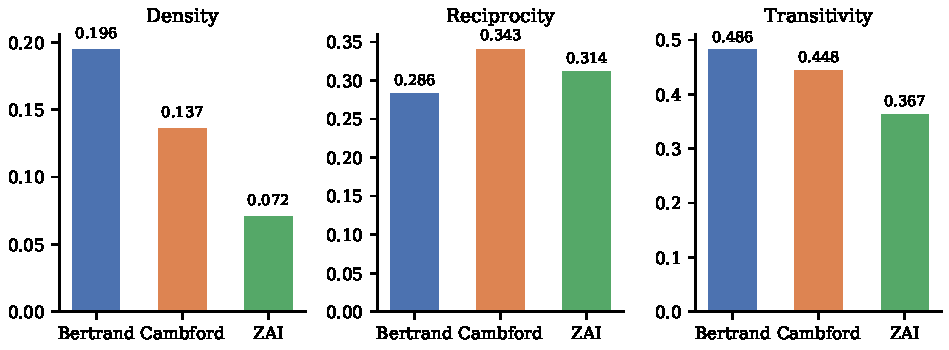
\includegraphics[width=0.85\linewidth]{figures/network_comparison.pdf}
\caption{Key communication-network metrics across the three EABench tenants. Density, reciprocity, and transitivity decrease with organizational scale, reflecting the transition from tight-knit professional-services firms to large engineering organizations with departmental silos.}
\label{fig:network_comparison}
\end{figure}

\noindent These metrics reflect realistic organizational archetypes. Bertrand \& Co., the smallest organization, is the densest (0.196) and has the smallest diameter (3), consistent with a tight-knit professional-services firm where most colleagues interact directly. ZAI Intelligence, the largest, exhibits a sparse, long-tail structure (density~0.072, 1{,}956 edges among 165~nodes) typical of rapidly growing technology companies with departmental silos. The University of Cambford occupies an intermediate position with the highest reciprocity (0.343), reflecting the collaborative back-and-forth characteristic of academic committee work. Transitivity is highest for Bertrand (0.486), where shared client matters create strong triadic closure, and lowest for ZAI (0.367), where cross-functional interaction is sparser.

The in-degree distributions follow a heavy-tailed pattern. We fit a power law $P(k) \sim k^{-\gamma}$ to the complementary cumulative distribution of in-degrees and compare the empirical graph against a synthetic Barab\'{a}si--Albert (BA) preferential-attachment graph of the same size. The low $\gamma$ values (0.36--0.68) confirm that all three networks exhibit right-skewed degree distributions rather than Poisson-like regularity. The $R^2$ values increase with tenant size (0.29 for Bertrand, 0.59 for ZAI), indicating that the power-law fit improves as the number of nodes permits a wider degree range. In each case, the maximum in-degree substantially exceeds the BA model's prediction (e.g., 99 vs.\ 72 for ZAI, 43 vs.\ 34 for Cambford), indicating that the generated organizations produce realistic ``hub'' individuals---such as executives, team leads, or central administrative staff---whose communication connectivity is disproportionately high.

Per-channel decomposition reveals further structural realism. Email communication has reciprocity between 0.48 and 0.73 across tenants, reflecting the natural tendency for emails to receive replies. Chat messages are entirely non-reciprocal at the edge level (0.0), since each message is a directed act from sender to recipient with no guaranteed return in the same thread. Meeting edges, constructed from attendee co-presence, are fully reciprocal by construction (1.0). This channel-level heterogeneity is important for evaluation: an agent that reasons about ``who communicated with whom'' must integrate evidence from channels with qualitatively different relational semantics.

\subsection{Temporal Communication Patterns}
\label{sec:temporal-stats}

Realistic enterprise datasets exhibit bursty temporal structure: communication tends to cluster around deadlines, incidents, or scheduled events rather than arriving as a uniform Poisson process. We quantify this using the burstiness parameter $B = (\sigma_\tau - \mu_\tau) / (\sigma_\tau + \mu_\tau)$, where $\mu_\tau$ and $\sigma_\tau$ are the mean and standard deviation of the inter-event time (IET) sequence for a given communication channel~\cite{goh2008burstiness}. Values of $B$ near zero indicate exponential (Poisson) inter-arrival times, while $B > 0$ indicates bursty clustering. We additionally report the memory coefficient $M$~\cite{goh2008burstiness}, which measures the correlation between consecutive IETs: $M > 0$ indicates that long gaps tend to follow long gaps (temporal clustering at multiple scales), while $M \approx 0$ indicates uncorrelated consecutive intervals.

\begin{table}[h]
\centering
\caption{Inter-event time (IET) statistics per communication channel and tenant.
Burstiness $B > 0$ indicates clustered arrivals; $B \approx 0$ indicates near-Poisson behavior.
Memory coefficient $M$ measures serial correlation between consecutive IETs.
$\alpha$ is the power-law exponent fitted to the IET distribution. Meeting channels are omitted for brevity (their $|B| < 0.01$ in all tenants except ZAI, where $B = 0.23$ with $M = 0.19$).}
\label{tab:iet_summary}
\small
\begin{tabular}{llccccc}
\toprule
\textbf{Tenant} & \textbf{Channel} & \textbf{Events} & \textbf{$B$} & \textbf{$M$} & \textbf{$\alpha$} & \textbf{Med.\ IET (s)} \\
\midrule
\multirow{3}{*}{Bertrand}
  & Email      & 132   & $-$0.051 & $-$0.054 & 2.00 & 81{,}450 \\
  & Chat (1:1) & 1{,}022 & $+$0.617 & $-$0.055 & 0.33 & 72       \\
  & Group Chat & 2{,}291 & $+$0.560 & $-$0.078 & 0.36 & 120      \\
\midrule
\multirow{3}{*}{Cambford}
  & Email      & 120   & $+$0.065 & $-$0.045 & 1.49 & 85{,}500 \\
  & Chat (1:1) & 732   & $+$0.640 & $-$0.048 & 0.35 & 90       \\
  & Group Chat & 2{,}075 & $+$0.575 & $-$0.072 & 0.34 & 110      \\
\midrule
\multirow{3}{*}{ZAI}
  & Email      & 298   & $+$0.168 & $+$0.395 & 1.28 & 82{,}800 \\
  & Chat (1:1) & 2{,}581 & $+$0.658 & $-$0.042 & 0.33 & 77       \\
  & Group Chat & 6{,}033 & $+$0.614 & $-$0.055 & 0.31 & 150      \\
\bottomrule
\end{tabular}
\end{table}

\noindent The results validate that EABench's generation pipeline reproduces two hallmarks of real organizational communication. First, email arrivals are near-Poisson ($B \approx 0$) across all three tenants, with high $\alpha$ values (1.28--2.00) indicating that inter-arrival times decay rapidly---consistent with the scheduled nature of formal correspondence. Second, chat and group-chat streams are highly bursty ($B \in [0.56, 0.66]$) with low power-law exponents ($\alpha \in [0.31, 0.36]$), confirming heavy-tailed inter-event time distributions where short bursts of rapid-fire messages are separated by long silences. This pattern matches empirical measurements of instant-messaging platforms in organizational settings~\cite{goh2008burstiness}.

The memory coefficients are near zero for most channel--tenant pairs ($M \in [-0.08, 0.0]$), indicating that the IET process is approximately memoryless at the single-channel level---as expected when daily narrative generation does not explicitly model autoregressive temporal dependence within a channel. The notable exception is ZAI's email channel ($M = +0.40$), where the organizational scale produces enough correlated event clusters (e.g., multi-day incident threads, product-launch email bursts) to induce measurable serial dependence.

This temporal structure directly impacts retrieval difficulty: an agent must reason about \emph{when} information was generated, not only \emph{what} it contains, because a correct multi-hop answer often depends on reconstructing an event sequence from artifacts whose timestamps are concentrated in bursty clusters rather than distributed uniformly.
